\title{Lab Assignment 2 \\ \small{Datamining}}
\author{Chiel ten Brinke 3677133}
\documentclass[12pt]{article}
\usepackage{amssymb,amsmath,amsthm,enumerate,graphicx,float,lmodern}

\newtheorem{theorem}{Theorem}[section]
\newtheorem{lemma}[theorem]{Lemma}
\newtheorem{proposition}[theorem]{Proposition}
\newtheorem{corollary}[theorem]{Corollary}

\theoremstyle{definition}
\newtheorem{definition}[theorem]{Definition}
\newtheorem{axiom}[theorem]{Axiom}
\newtheorem{example}[theorem]{Example}
\newtheorem{remark}[theorem]{Remark}

\newcommand{\set}[2]{\left\lbrace#1 \, \middle|\, #2 \right\rbrace}

\begin{document}
\maketitle

\section*{Data Analysis}
\label{sec:data_analysis}

\paragraph{Note}
The Bron-Kerbosch algorithm has not been taken from the site, but has been implemented manually.

\subsection*{a}
There are 10 variables, so there are $\frac{10 \cdot 9}{2} = 45$ undirected edges.
Since each combination of edges represents exactly one graphical model,
there are $2^{45} = 35184372088832$ possible graphical models.

\subsection*{b}
The table of counts has a cell for each combination of variable values.
This comes down to $9 \cdot 2 \cdot 2 \cdot 2 \cdot 3 \cdot 6 \cdot 4 \cdot 3 \cdot 5 \cdot 2 = 155520$ possible combinations.
This is confirmed by taking the length function of the table of counts in R.
The number of parameters of the saturated model equals the number of cells in the table of counts.

\subsection*{c}
Cliques: 

\subsection*{h}
To get a first impression of how the parameters nstart and prob relate to the score functions,
let us perform series of small tests for varying parameters and construct a graph from this.
To keep the compution time within reasonable bounds, we work with a randomly sampled subset
from the original dataset.
Moreover, we will not consider all 10 variables during the hill climbing part, but only a subset.
For each configuraton of the parameters, we run the hill climbing algorithm 10 times with 4
randomly chosen variables.
The average score of these runs is taken to be the final outcome for this configuraton.

\begin{figure}[H]
    \centering
    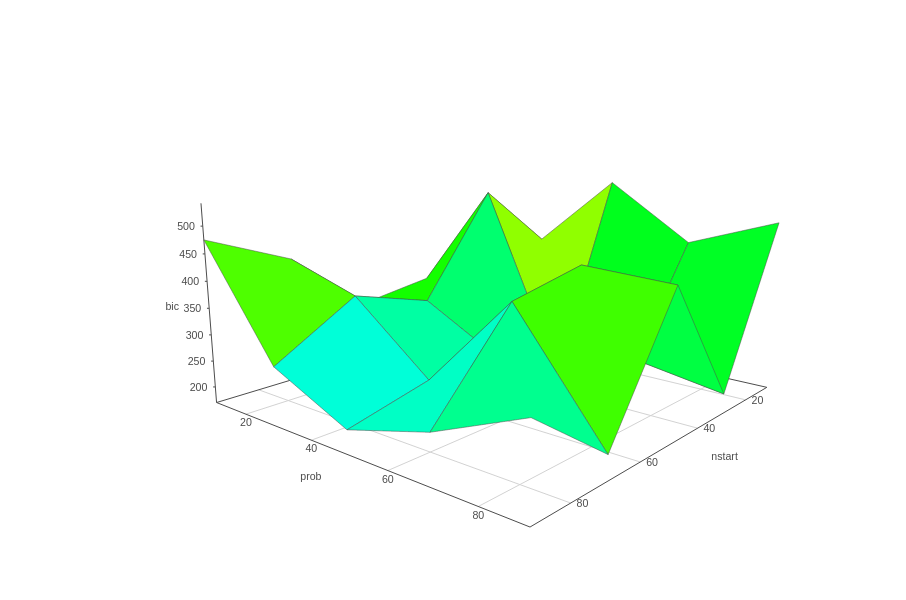
\includegraphics[width=0.8\linewidth]{rough2.png}
    \caption{BIC score as a function of nstart and prob.}
\label{fig:rough}
\end{figure}


\begin{table}[h]
\centering
\begin{tabular}{lll}
    nstart & prob & AIC \\
    \hline \hline
    10 & 0.5  & 0.0966667 \\
\end{tabular}
\caption{AIC score as a function of nstart and prob.}
\label{table1}
\end{table}

\begin{table}[h]
\centering
\begin{tabular}{lll}
    nstart & prob & BIC \\
    \hline \hline
    10 & 0.5  & 0.0966667 \\
\end{tabular}
\caption{BIC score as a function of nstart and prob.}
\label{table1}
\end{table}

\end{document}
